\chapter{Literature Review}
\label{ch:LiteratureReview}

\section{Image Quality Assessment (IQA)}
\label{sec:OverviewTeledermatology}
This section delves into the fundamentals of Image Quality Assessment (IQA), a field dedicated to the objective quantification of image quality. IQA plays a critical role in evaluating the fidelity, clarity, and other essential quality aspects of images, utilizing a variety of metrics specifically designed for these purposes. \par
\vspace{\baselineskip}
Image Quality Assessment is crucial for identifying various forms of image degradation, which can include blurring, geometric distortions (such as shrinking or zooming), and blockiness artifacts often resulting from compression standards. The primary goal of IQA is to quantify these degradations accurately, thereby ensuring the fidelity and perceptual quality of images. This process involves a rigorous assessment that helps maintain the integrity and usability of images across different applications and platforms.\par
\vspace{\baselineskip}
Moreover, IQA often intersects with other areas of image assessment. For example, Image Aesthetics Assessment, which focuses on the visual appeal of images as perceived by human observers, shares common tools and objectives with IQA. Similarly, Image Fidelity Assessment deals with how accurately a reconstructed image represents the original scene, a concern that is closely linked to the core pursuits of IQA. These connections highlight the broad applicability and relevance of IQA methods in various domains, including those beyond traditional technical analysis, emphasizing the importance of developing robust IQA techniques.\par
\vspace{\baselineskip}
In addition to discussing these fundamental concepts, this section will review benchmark datasets commonly used in IQA research and explore state-of-the-art (SOTA) methods currently leading the field. This exploration not only provides a comprehensive background of IQA but also sets the stage for applying these methods and principles specifically to the challenges faced in teledermatology.\par

\subsection{Subjective Quality Assessment}
\label{sub:SubjectiveQualityAssessment}
Subjective quality assessment refers to the process where human observers evaluate the quality of images based on their visual perception. This method is integral to understanding how humans perceive image quality in practical scenarios, including scenarios where technical measures might not fully capture the perceived quality. There are two primary methods utilized in subjective quality assessment:\par
\begin{itemize}
    \item Absolute Categorical Rating:  In this approach, human observers are presented with an image and asked to rate its quality based on predefined categories. Each observer evaluates the image independently, without comparing it to any reference image. This method allows assessors to provide a direct judgment on the image's quality based on their subjective experience.
    \item Paired Comparison: Here, human observers are presented with two images: the test image and a reference image. Observers then assess the quality of the test image by comparing it directly to the reference image, assigning a score based on the perceived differences in quality. However, the paired comparison method is less applicable in teledermatology because a standard reference image is usually not available, especially since the exact condition depicted in the patient's image may not be known.
\end{itemize}
Subjective quality assessment is highly valued for its ability to accurately reflect human perception of image quality. However, this method is also resource-intensive, requiring significant time and effort from human assessors. Moreover, subjective assessments can be susceptible to variability and biases introduced by individual scorers, which can affect the consistency and reliability of the evaluations. Despite these challenges, subjective quality assessment remains a critical component of comprehensive image quality evaluation, particularly in applications where the human response to an image is the ultimate measure of its quality.\par

\subsection{Objective Quality Assessment}
\label{sub:ObjectiveQualityAssessment}
Objective quality assessment relies on mathematical algorithms rather than human judgment to evaluate image quality. This approach is categorized mainly into three methods, each differing based on the reference data used during the evaluation: Full-Reference IQA (FR-IQA), Reduced-Reference IQA (RR-IQA), and No-Reference IQA (NR-IQA). \par
\vspace{\baselineskip}
\begin{figure}[ht]
    \centering
    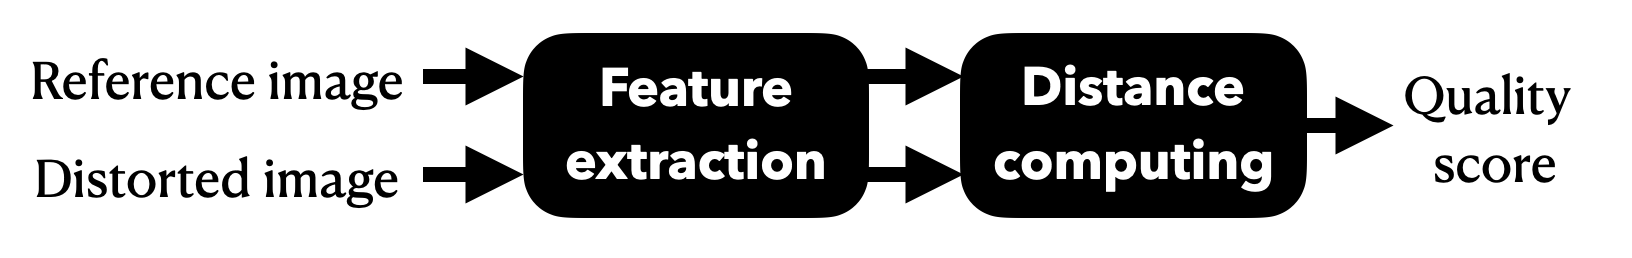
\includegraphics[keepaspectratio,width=15cm]{img/FRIQA.png}
    \caption{Comparison between a distorted image and a reference image to compute quality scores.}
    \label{fig:FRIQA}
\end{figure}
\textbf{Full-Reference IQA (FR-IQA)} \ref{fig:FRIQA}  involves a comprehensive comparison between a distorted image and a reference image. In this method, features are extracted from both the distorted and the reference image, and their differences are quantitatively analyzed to compute a quality score. FR-IQA offers a detailed assessment of image quality but requires the availability of a reference image for every distorted image evaluated, which can sometimes limit its applicability. \par
\vspace{\baselineskip}
\begin{figure}[ht]
    \centering
    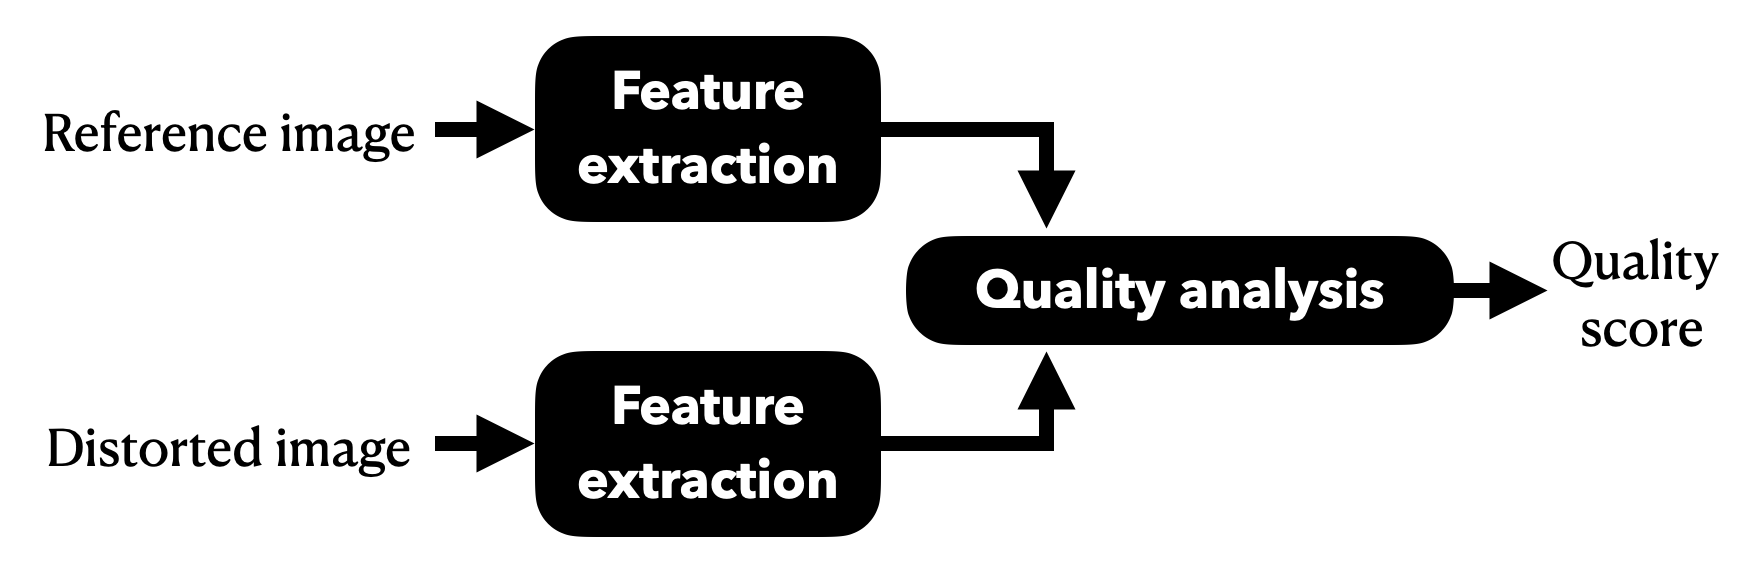
\includegraphics[keepaspectratio,width=15cm]{img/RRIQA.png}
    \caption{Reduced-reference assessment comparing features extracted from distorted and reference images for quality analysis.}
    \label{fig:RRIQA}
\end{figure}
\textbf{Reduced-Reference IQA (RR-IQA)} \ref{fig:RRIQA} operates under a similar principle to FR-IQA but does not require the complete reference image. Instead, it uses a reduced set of features extracted from both the distorted and reference images. This method strikes a balance between the exhaustive comparison of FR-IQA and the complete independence of NR-IQA, reducing computational demands while still providing meaningful quality assessments based on partial reference data. \par
\vspace{\baselineskip}
Both FR-IQA and RR-IQA utilize two methods to analyze quality:
\begin{itemize}
    \item Spatial-Based Analysis: This method compares images pixel by pixel or region by region, providing straightforward interpretation and efficient computation. However, it may lack robustness and does not fully align with how the human visual system processes images.
    \item Transform-Based Analysis:This approach transforms images into a different domain (like the frequency domain) that more closely mimics the human visual system. While providing robust assessments, it is complex and computationally intensive.
\end{itemize}
\vspace{\baselineskip}
\begin{figure}[ht]
    \centering
    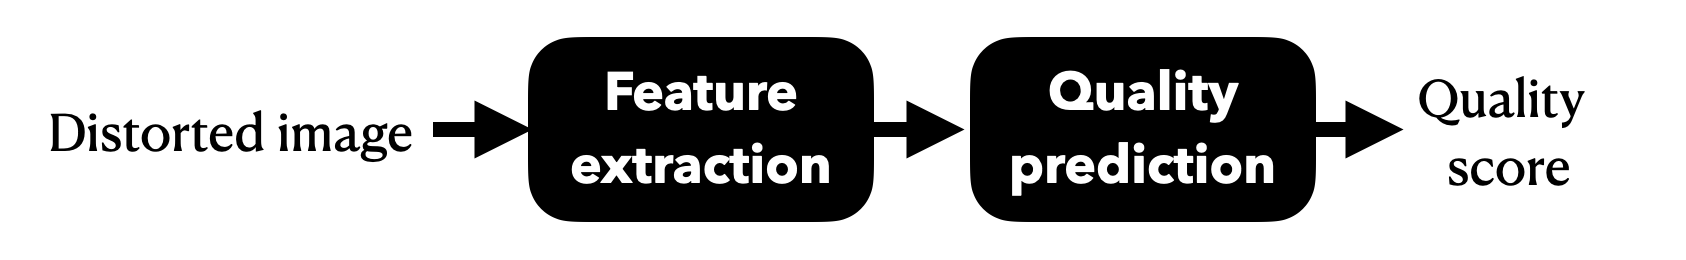
\includegraphics[keepaspectratio,width=15cm]{img/NRIQA.png}
    \caption{Quality assessment based solely on features extracted from the distorted image, without a reference image.}
    \label{fig:NRIQA}
\end{figure}

\textbf{No-Reference IQA (NR-IQA)} \ref{fig:NRIQA} is the third category, which does not rely on any reference image. Instead, it analyzes the distorted image alone by extracting features that are indicative of quality. This method is particularly useful in situations where no reference images are available, such as in many practical applications of teledermatology. NR-IQA can be tailored to address specific types of distortions or designed for general-purpose quality assessment, providing versatility across various domains. \par
\vspace{\baselineskip}
For this thesis, the focus will be on NR-IQA, especially considering its relevance in evaluating teledermatology images where reference images are not typically available. This focus on NR-IQA aims to enhance the robustness and applicability of quality assessment in real-world teledermatology scenarios, addressing the diverse and specific challenges encountered in this field.

\subsection{Common Distortions in IQA}
\label{sub:CommonDistortionsIQA}
Image Quality Assessment (IQA) must address various distortions that can significantly affect the perceived quality of images. Understanding these common distortions is essential for developing effective IQA algorithms, particularly in contexts like teledermatology where accurate image assessment is critical. Here are the primary distortions typically considered in IQA: \par
The common distortions are \cite{https://arxiv.org/abs/2310.14918}:
\begin{figure}[ht]
    \centering
    \begin{subfigure}[b]{0.24\textwidth}
        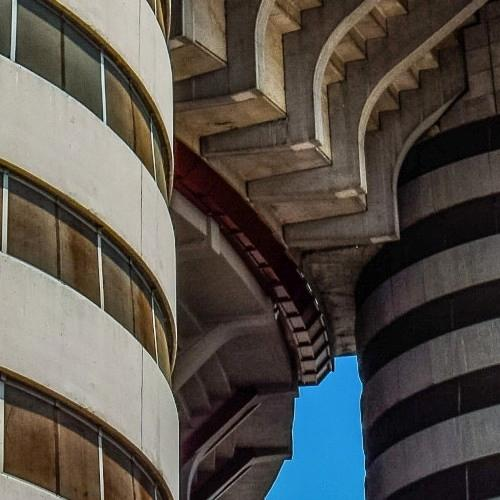
\includegraphics[width=\textwidth]{img/Original.jpg}
        \caption{Original}
    \end{subfigure}
    \hfill
    \begin{subfigure}[b]{0.24\textwidth}
        
\includegraphics[width=\textwidth]{img/Blur.jpg}
        \caption{Blur}
        \label{fig:blur}
    \end{subfigure}
    \hfill
    \begin{subfigure}[b]{0.24\textwidth}
        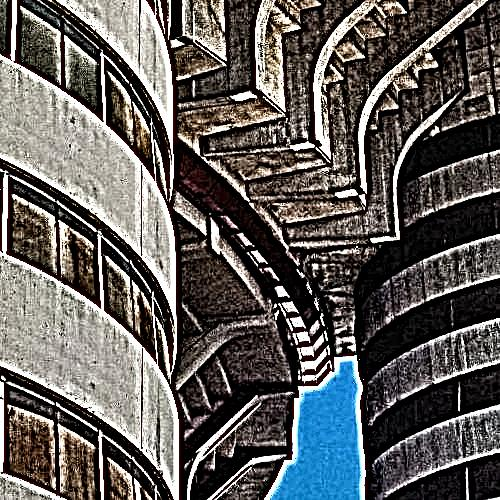
\includegraphics[width=\textwidth]{img/Sharpness.jpg}
        \caption{Sharpness}
        \label{fig:sharpness}
    \end{subfigure}
    \hfill
    \begin{subfigure}[b]{0.24\textwidth}
        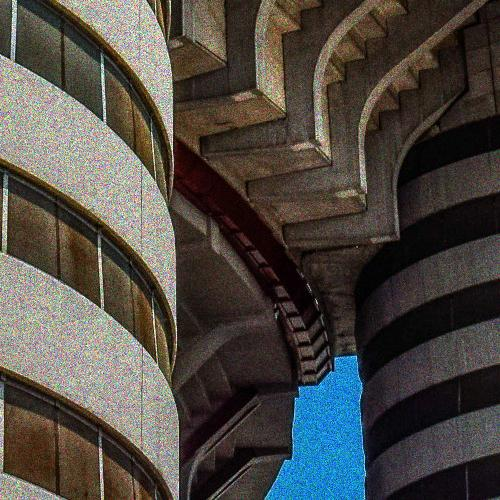
\includegraphics[width=\textwidth]{img/Noise.jpg}
        \caption{Noise}
        \label{fig:noise}
    \end{subfigure} 

    \begin{subfigure}[b]{0.24\textwidth}
        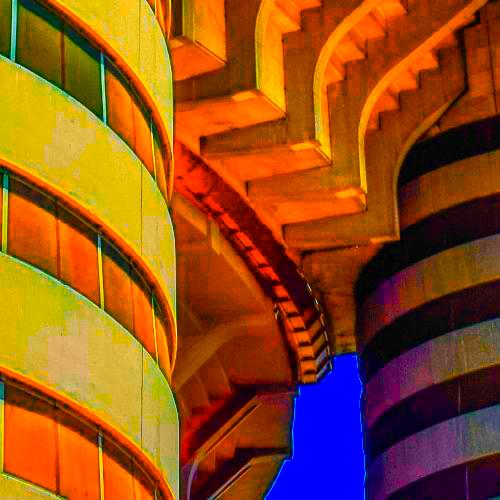
\includegraphics[width=\textwidth]{img/ColorAccuracy.jpg}
        \caption{Color Accuracy}
        \label{fig:color_accuracy}
    \end{subfigure}
    \hfill
    \begin{subfigure}[b]{0.24\textwidth}
        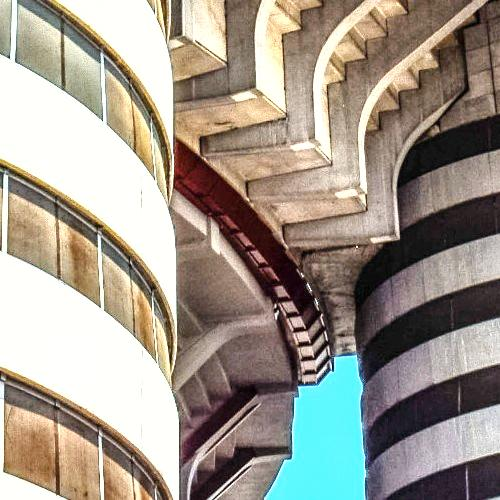
\includegraphics[width=\textwidth]{img/BrightnessContrast.jpg}
        \caption{Brightness \& Contrast}
        \label{fig:brightness_contrast}
    \end{subfigure}
    \hfill
    \begin{subfigure}[b]{0.24\textwidth}
        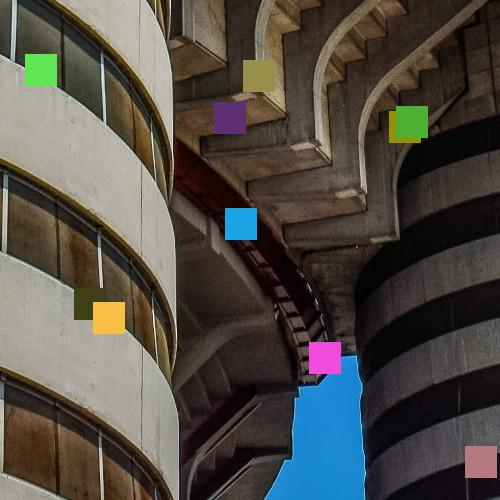
\includegraphics[width=\textwidth]{img/Artifacts.jpg}
        \caption{Artifacts}
        \label{fig:artifacts}
    \end{subfigure}
    \hfill
    \begin{subfigure}[b]{0.24\textwidth}
        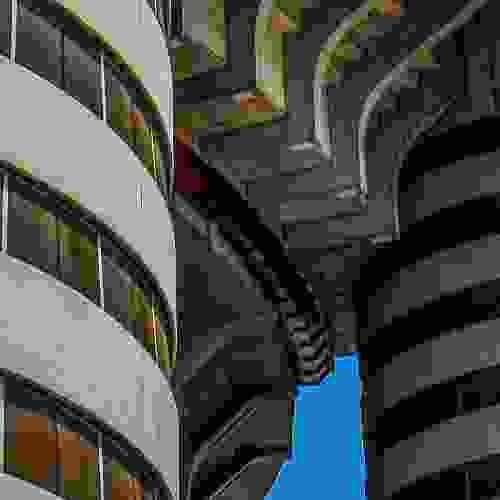
\includegraphics[width=\textwidth]{img/Compression.jpg}
        \caption{Compression}
        \label{fig:compression}
    \end{subfigure}
    \caption{Example images illustrating common distortions used in Image Quality Assessment.}
    \label{fig:distortions}
\end{figure}
\begin{enumerate}
    \item \textbf{Blur}: Blurred images lack sharpness and clarity, often resulting from motion during capturing, incorrect focus settings, or imperfections in the camera lens. Example lens blured image: \ref{fig:blur}.
    \item \textbf{Sharpness}: Sharpness refers to how well-defined the edges and fine details in an image appear. High sharpness is indicative of clear, crisp images, whereas a lack of sharpness can make an image look soft and unclear. Example high sharpened image: \ref{fig:sharpness}.
    \item \textbf{Noise}: Noise appears as random variations in brightness or color in an image and is often due to the limitations of the camera's sensor, particularly under low light conditions or at high ISO settings. Example white noise image: \ref{fig:noise}.
    \item \textbf{Color Accuracy}: Color accuracy pertains to the faithful reproduction of colors in an image. Distortions in color accuracy can lead to inaccurate or unrealistic color representation. Example saturated image: \ref{fig:color_accuracy}.
    \item \textbf{Brightness \& Contrast}: Brightness is the overall light level of an image, while contrast refers to the range between its darkest and lightest areas. Proper balance of both is crucial for maintaining image visibility and detail. Excessive or insufficient brightness and contrast can render an image unusable for detailed analysis. Example brightened image: \ref{fig:brightness_contrast}.
    \item \textbf{Artifacts}: Artifacts are unwanted visual anomalies introduced during image acquisition or processing, such as halos, or jagged edges. Example artifact in image: \ref{fig:artifacts}.
    \item \textbf{Compression}: When images are compressed to reduce file size, this often results in lost detail and visible quality degradation. Example JPEG compressed image: \ref{fig:compression}.
\end{enumerate}
Each distortion type affects the visual quality and perceptual fidelity of images, influencing the effectiveness of IQA methodologies in assessing image quality. Understanding these distortions is crucial for developing robust quality assessment algorithms and enhancing image fidelity in various applications, including teledermatology.

\subsection{Benchmark Datasets for IQA}
\label{sub:BenchmarkDatasetsIQA}
Benchmark datasets are crucial for advancing the field of Image Quality Assessment (IQA) by providing standardized and diverse image sets with known distortions and corresponding quality annotations. These annotations, primarily in the form of Mean Opinion Score (MOS) and Differential Mean Opinion Score (DMOS), serve as reference points for evaluating the performance of IQA algorithms. \par
\vspace{\baselineskip}
\textbf{Mean Opinion Score (MOS)} is a measure obtained by averaging the ratings provided by human observers for the perceived quality of images on a predefined scale. This metric reflects the overall perceptual quality as judged by typical viewers and is used extensively to assess the performance of IQA methods against human visual judgment. \par
\vspace{\baselineskip}
\textbf{Differential Mean Opinion Score (DMOS)}, on the other hand, is derived from MOS but focuses on the perceptual difference in quality between a reference image and a distorted version. DMOS is particularly useful in scenarios where the impact of specific distortions on perceived image quality needs to be quantified. \par
\vspace{\baselineskip}
The availability of these datasets allows researchers to thoroughly test the robustness, accuracy, and generalization capabilities of various IQA methodologies. Furthermore, they support the development of innovative algorithms by offering ground-truth quality scores, crucial for fostering reproducible research practices. \par

\subsubsection{Datasets Commonly Used in IQA}
\label{subsub:DatasetsIQA}

\begin{table*}[!t]
    \centering
    \caption{An overview of IQA databases}
    \label{tab:iqa_databases}
    \renewcommand{\arraystretch}{1.5}
    \resizebox{\textwidth}{!}{ % Resize table to fit within the text width
    \begin{tabular}{p{2.3cm} p{2cm} c c c p{3.5cm} c  p{2.3cm} c}
    \toprule
        Category & Database & Year & \#Ref. & \#Dist. & \#Dist. Type & \#Dist. Level & Resolution Type & Ground-truth \\
        \hline
        \multirow{8}{*}{General} 
        & LIVE \cite{LIVE} & 2004 & 30 & 779 & JPEG, JP2K, WN, GB, FF& 5 or 4 & 768 $\times$ 512 & DMOS \\
        & TID2008 \cite{TID2008} & 2008 & 25 & 1700 & 17 & 4 & 512 $\times$ 384 & MOS \\
        & TID2013 \cite{TID2013} & 2013 & 25 & 3000 & 24 & 5 & 512 $\times$ 384 & MOS \\
        & CSIQ \cite{CSIQ} & 2009 & 30 & 866 & JPEG, JP2K, WN, GB, APGN,  GCD & 5 or 4 & 512 $\times$ 512 & DMOS \\
        & A57 \cite{A57} & 2007 & 3 & 54 & 6 & 3 & 512 $\times$ 512 & MOS \\
        & WED \cite{WED} & 2017 & 4744 & 94880 & JPEG, JP2K, GB, WN& 5 & - & - \\
        & KADIS700K \cite{KADIS700K} & - & - & - & - & - & - & - \\
        & KADID \cite{KADID} & - & - & - & - & - & - & - \\
        \hline
        \multirow{3}{*}{Multiple Dist.} 
        & LIVEMD \cite{LIVEMD} & 2012 & 15 & 405 & GB followed by JPEG, GB followed by WN& - & 1280 $\times$ 720 & DMOS \\
        & MDID2013 \cite{MDID2013} & 2013 & 12 & 324 & corrupted successively by GB, WN, and JPEG& - & 768 $\times$ 512 or 1280 $\times$ 720 & DMOS \\
        & MDID2016 \cite{MDID2016} & 2016 & 20 & 1600 & GB or CC first, JPEG or JP2K second and WN last& - & 512 $\times$ 384 & MOS \\
        \hline
        \multirow{4}{*}{Screen content} 
        & SIQAD \cite{SIQAD} & 2014 & 20 & 980 & WN, GB, CC, JPEG, JP2K, MB, LSBC& 7 & 700 $\times$ 700 & DMOS \\
        & SCIQ \cite{SCIQ} & 2017 & 40 & 1800 & WN, GB, MB, CC, JPEG, JP2K, CSC, CQD& 5 & 1280 $\times$ 720 & MOS \\
        & CCT \cite{CCT} & 2017 & 72 & 1320 & HEVC and HEVC-SCC coding& 11 & 1280 $\times$ 720 to 1920 $\times$ 1080 & MOS \\
        & HSNID \cite{HSNID} & 2019 & 20 & 600 & WN, GB, MB, CC, JPEG, JP2K& 5 &  - & MOS \\
        \hline
        \multirow{2}{*}{Authentic Dist.} 
        & LIVE Wild \cite{LIVEWild} & 2016 & 0 & 1162 & - & - & 500 $\times$ 500 & MOS \\
        & CID2013 \cite{CID2013} & 2015 & 0 & 480 & - & - & 1600 $\times$ 1200 & MOS \\
    \bottomrule
    \end{tabular}
    }
    \raggedright
    \scalebox{0.59}{
    \begin{tabular}{l}
        Note: \#Ref.: Total number of pristine images. \quad \#Dist.: Total number of distorted images. \quad JPEG: JPEG compression. \quad JP2K: JPEG2000 compression. \\ 
         \quad  \quad  \quad WN.: White noise. \quad GB: Gaussian blur. \quad FF: Simulated fast fading Rayleigh channel. \quad CSC: Color saturation change. \quad CC: Contrast change. \\
         \quad  \quad  \quad CQD: Color quantization with dithering. \quad APGN: Additive pink Gaussian noise. \quad GCD: Global contrast decrements. \quad MB.: motion blue. \\ 
         \quad  \quad  \quad LSBC.: Layer segmentation based compression. \quad HEVC-SCC: Screen content coding extension of high efficiency video coding. 
    \end{tabular}
    }
\end{table*}

\vspace{\baselineskip}
\begin{itemize}
    \item \textbf{LIVE} (Laboratory for Image \& Video Engineering) dataset (\cite{LIVE}) includes 29 reference images and 779 manually distorted images corrupted by 5 types of distortions: JPEG compression (JPEG), JPEG2000 compression (JP2K), white noise (WN), Gaussian blur (GB), and simulated fast fading Rayleigh channel (FF). Each distortion type contains 5 or 4 distortion levels. Most images are 768 $\times$ 512 pixels in size. Each distorted image in this dataset is associated with a Differential Mean Opinion Score (DMOS), scaled from 0 to 100, where 0 indicates no perceivable distortion. 
    \item \textbf{TID2008} (Tampere image database 2008) dataset (\cite{TID2008}) includes 25 reference images and 1700 distorted images corrupted by 17 types of distortions, with 4 levels for each distortion type. All images have a fixed resolution of 512 $\times$ 384. This dataset provides MOS values and their standard deviations, with MOS ranging from 0 to 9, where 9 signifies a distortion-free image.
    \item \textbf{TID2013} (Tampere image database 2013) dataset (\cite{TID2013}) is extended from TID2008 (\cite{TID2008}) by increasing the number of distortion levels to 5, and the number of distortion types to 24. Therefore, 3000 distorted images are generated from 25 pristine images. The subjective testing and data processing steps are similar to that of TID2008. DMOS values for this dataset were derived from over half a million ratings given by nearly a thousand observers, with values ranging from 0 to 9, where higher values denote poorer image quality.
    \item \textbf{CSIQ} (Categorical subjective image quality (CSIQ) database) (\cite{CSIQ}) contains 30 pristine images and 866 distorted images corrupted by JPEG, JP2K, WN, GB, additive pink Gaussian noise, and global contrast decrements, with 5 or 4 levels for each distortion type. The resolution is 512 $\times$ 512. Each image in CSIQ is associated with DMOS values obtained from subjective ratings by 25 testers, with DMOS values scaled from 0 to 1, where higher values indicate worse quality.
    \item \textbf{A57} (\cite{A57}) includes 3 pristine images and 54 distorted images corrupted by 6 types of distortions, with 3 levels for each distortion type. All images are in gray scale. The resolution is 512 $\times$ 512. \todo{search database and maybe add KonIQ-10k and other from ARNIQA!}
    \item \textbf{WED} (Waterloo exploration database) (\cite{WED}) includes 4744 pristine natural images and 94880 distorted images corrupted by JPEG, JP2K, GB, and WN, with 5 levels for each distortion type. The images have various resolutions. No human opinion score is provided, but the authors introduce several alternative test criteria to evaluate the IQA models.
\end{itemize}

\textbf{Multiple Distortions IQA Databases}
\begin{itemize}
    \item \textbf{LIVEMD} (LIVE multiply distorted) (\cite{LIVEMD}) database consists of 15 reference images and 405 multiply distorted images. The database includes one/double-fold artifacts. Each multiply distorted image is corrupted under two multiple distortion scenarios: Gaussian blur followed by JPEG and Gaussian blur followed by white noise. All images have a resolution of 1280 $\times$ 720. DMOS values for each distorted image range from 0 to 100.
    \item \textbf{Multiply distorted image database 2013 (MDID2013)} \cite{MDID2013}: MDID2013 has a total of 12 pristine images and 324 distorted images. Each pristine image is corrupted successively by Gaussian blur, white noise, and JPEG. The images have resolutions of 768 $\times$ 512 or 1280 $\times$ 720.
    \item \textbf{Multiply distorted image database 2016 (MDID2016)} \cite{MDID2016}: MDID2016 consists of 20 reference images and 1600 distorted images. Five distortion types are introduced, i.e., white noise, Gaussian blur, JPEG, JPEG2000, and contrast change (CC). The order of distortions is as follows: Gaussian blur or CC first, JPEG or JPEG2000 second, and white noise last. All distorted images are with random types and levels of distortions. The image resolution is 512 $\times$ 384.
\end{itemize}

\textbf{Screen Content IQA Databases}
\begin{itemize}
    \item \textbf{Screen Image Quality Assessment Database (SIQAD)} \cite{SIQAD}: SIQAD includes 20 pristine and 980 distorted screen content images (SCIs). Distortion types include white noise (WN), Gaussian blur (GB), color cast (CC), JPEG, JPEG2000 (JP2K), motion blur (MB), and layer segmentation-based compression, with 7 levels for each type. The images have various resolutions near 700 $\times$ 700.
    \item \textbf{Screen Content Image Quality (SCIQ) Database} \cite{SCIQ}: SCIQ consists of 40 pristine and 1800 distorted SCIs corrupted by 9 types of distortions, including WN, GB, MB, CC, JPEG, JP2K, color saturation change (CSC), color quantization with dithering (CQD), and the screen content coding extension of High Efficiency Video Coding (HEVC-SCC). Five distortion levels are considered. The resolution is fixed at 1280 $\times$ 720.
    \item \textbf{Cross-Content-Type (CCT) Database} \cite{CCT}: CCT is constructed to conduct cross-content-type IQA research. CCT consists of 72 pristine and 1320 distorted natural scene images (NSIs), computer graphic images (CGIs), and SCIs. Two distortion types are considered, i.e., HEVC and HEVC-SCC coding, with 11 distortion levels for each type. The image resolution is either 1920 $\times$ 1080 or 1280 $\times$ 720.
    \item \textbf{Hybrid Screen Content and Natural Scene Image Database (HSNID)} \cite{HSNID}: HSNID has 10 pristine NSIs and 10 pristine SCIs, and 600 distorted NSIs and SCIs corrupted by WN, GB, MB, CC, JPEG, and JP2K, with 5 distortion levels for each type.
\end{itemize}

\textbf{Authentic Distortions IQA Databases}
\begin{itemize}
    \item \textbf{LIVE in the wild image quality challenge database} \cite{LIVEWild} includes 1162 authentically distorted images captured using a variety of mobile devices. Complex real distortions, which are not well-modeled by the synthetic distortions are included. All images are cropped to the resolution of 500 $\times$ 500. A novel crowdsourcing system was employed to gather over 350,000 opinion scores from 8100 observers, ensuring the objectivity of the MOS values obtained.
    \item \textbf{Camera image database (CID2013)} \cite{CID2013}: CID2013 is designed to test no-reference IQA algorithms. It includes 480 real images captured from 8 typical scenes using 79 consumer cameras and mobile phones. The images are rated from 5 aspects: the overall quality, sharpness, graininess, lightness, and color saturation scales. The images are scaled to a size of 1600 $\times$ 1200.
\end{itemize}

\subsection{State-of-the-Art in IQA}
\label{sub:SOTA_IQA}
The current state-of-the-art (SOTA) in Image Quality Assessment (IQA) within the general image domain is ARNIQA. ARNIQA (leArning distoRtion maNifold for Image Quality Assessment) represents a significant advancement in No-Reference Image Quality Assessment (NR-IQA), which aims to objectively measure image quality in a way that aligns with human perception, even in the absence of a high-quality reference image. This is particularly crucial in applications such as teledermatology, where the quality of diagnostic images directly impacts the accuracy of the assessments made by healthcare professionals.\par
\subsubsection{Overview ARNIQA}
\label{subsub:OverviewARNIQA}
ARNIQA is developed as a self-supervised approach that learns the image distortion manifold, which is a comprehensive model of all possible image degradations. This learning approach is designed to maximize the similarity between embeddings of differently contented images that share similar distortion levels. Such a strategy allows ARNIQA to focus on the quality and type of distortions rather than the content itself, enhancing its applicability across different domains where specific content can vary widely.\par
\begin{figure}[ht]
    \centering
    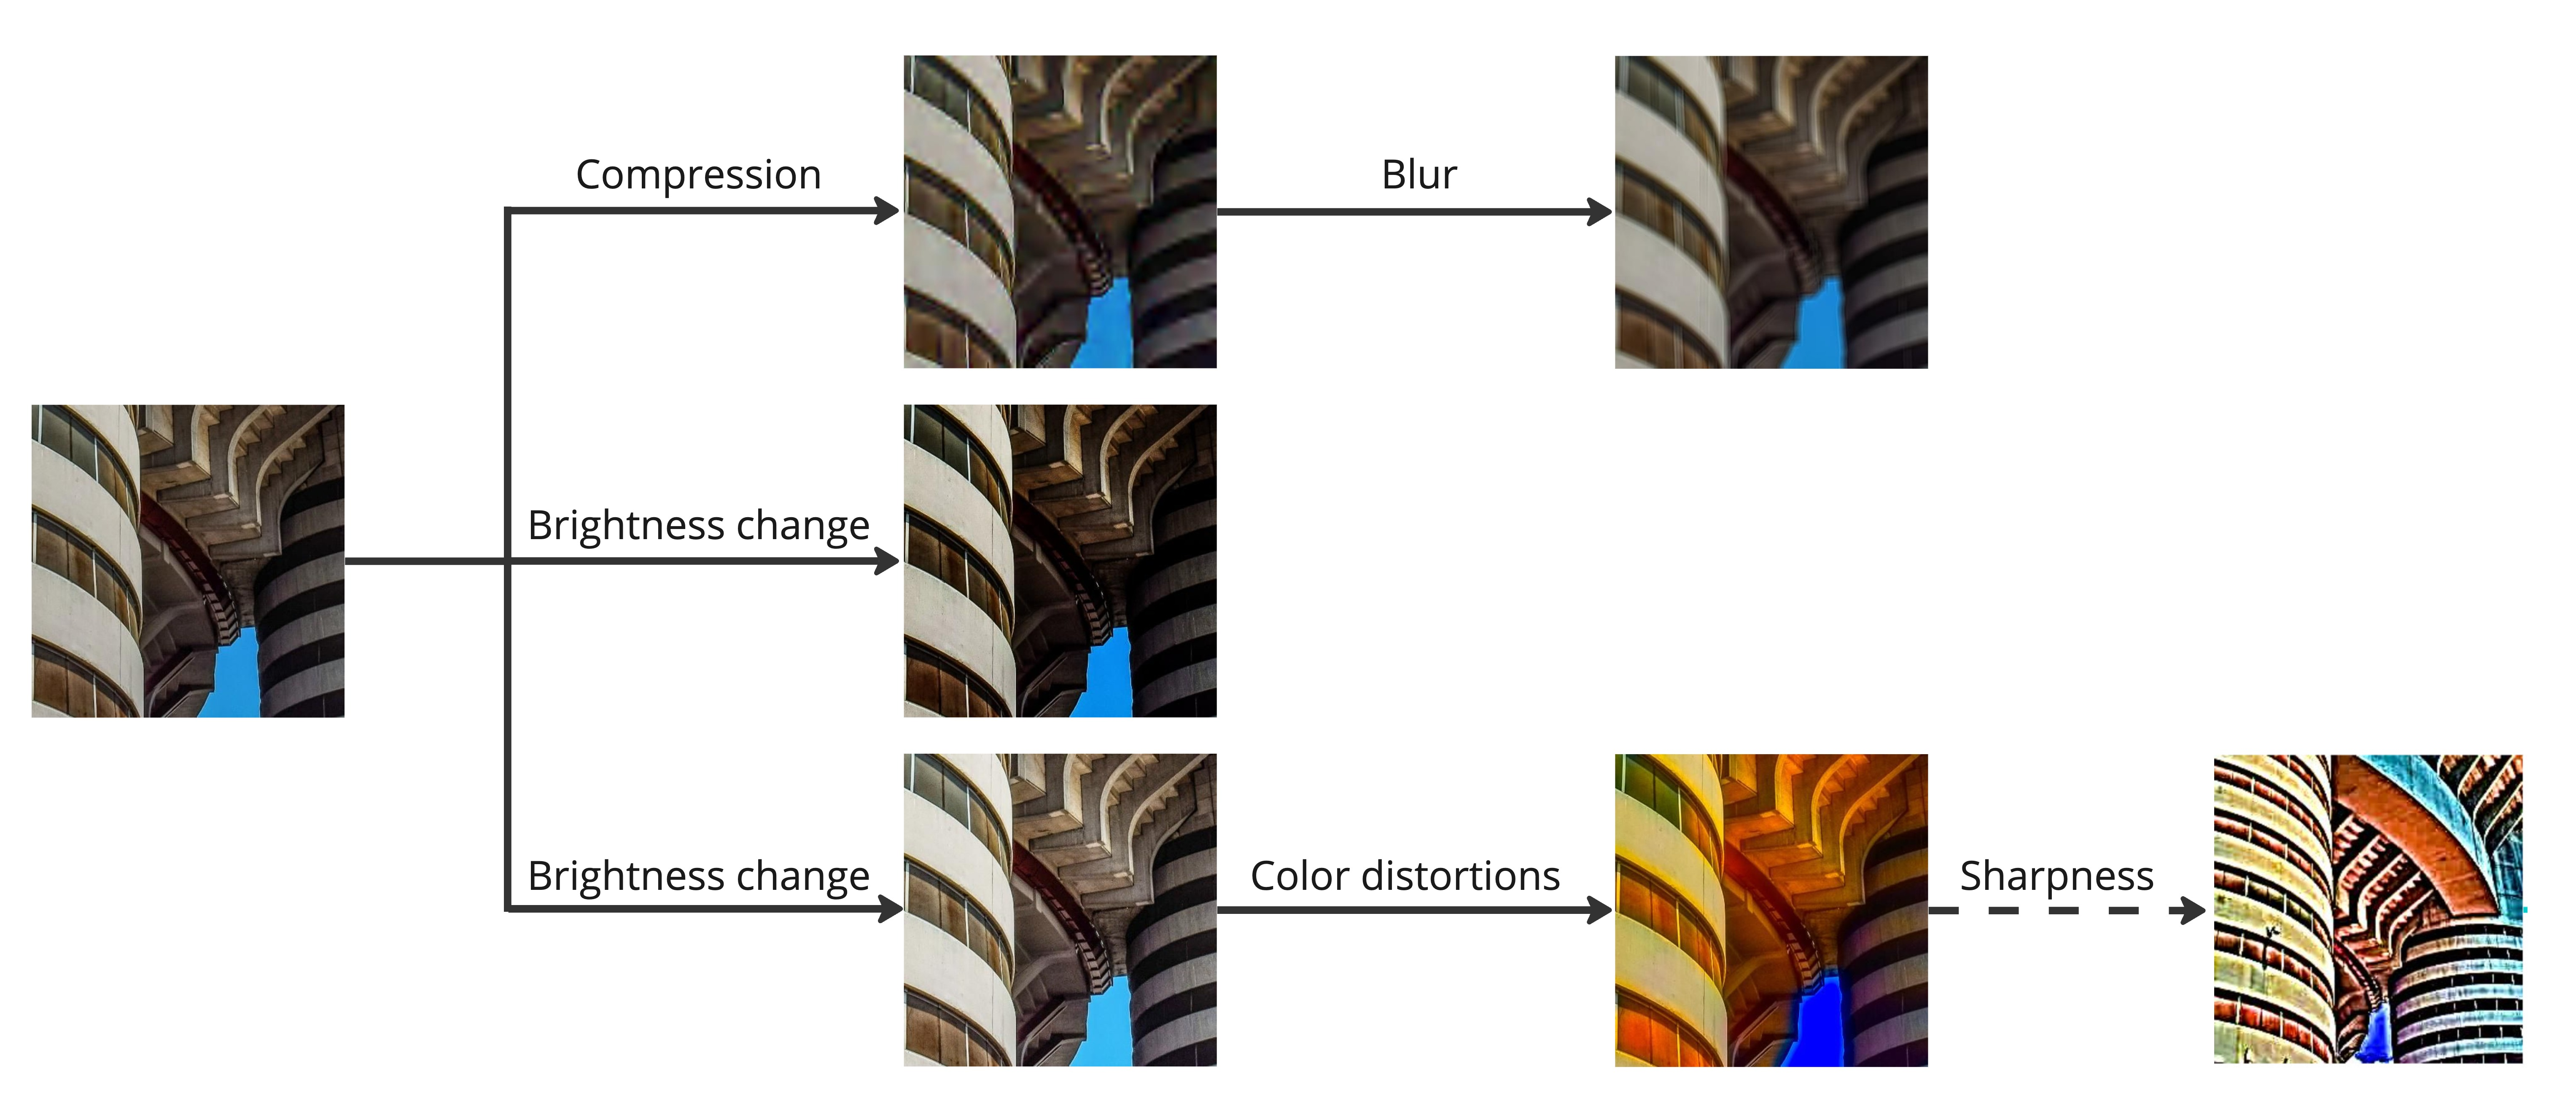
\includegraphics[keepaspectratio,width=15cm]{img/degradation.jpg}
    \caption{Overview of the image degradation model from ARNIQA. Where they randomly assemble distortion compositions in ordered sequences of distortions applied consecutively, to synthetically generate images with a wide variety of degradation patterns. Each distortion composition sampled from 7 distinct distortion groups.}
    \label{fig:ARNIQAdegradation}
\end{figure}
The model includes an innovative image degradation model that can synthesize images with a sequence of up to 100 times more distinct combinations of distortions compared to existing methods. This capability is critical as it allows for extensive training and robust model performance across a wide array of real-world distortions encountered in practical applications.\par
\vspace{\baselineskip}
\noindent
\textbf{Training Strategy of ARNIQA}: ARNIQA’s training strategy involves two main phases:\par
\noindent
\begin{enumerate}
    \item Encoder Pre-training: The model uses a large set of unlabeled images that are synthetically degraded. This step allows the encoder to learn a diverse set of image features associated with different types and levels of quality degradation.
    \item Regressor Training: A dataset-specific linear regressor is then trained using the Mean Opinion Scores (MOS) of images. This regressor is responsible for mapping the learned image features to actual quality scores, enabling the model to predict the perceived image quality accurately.
\end{enumerate}
\textbf{Self-Supervised Learning}: The self-supervised learning component is particularly significant because it circumvents the need for extensively labeled data sets, which are often costly and time-consuming to develop. By relying on synthetically degraded images for which quality parameters are already known, ARNIQA can train effectively without human-labeled data. \par
\vspace{\baselineskip}
\noindent
\textbf{Performance and Generalization}: ARNIQA has demonstrated superior performance and generalization capabilities over competing methods. Its robustness in handling a wide range of distortion types and severities makes it an excellent choice for applications like teledermatology, where images must be assessed for quality in a highly variable environment. \par
\vspace{\baselineskip}
\noindent
ARNIQA comprises three main components: 
\par
\vspace{\baselineskip}
\noindent
\textbf{Image Degradation Model}: ARNIQA includes a sophisticated image degradation model that can synthetically degrade images through a combination of up to 1.9 billion distinct degradation patterns. This model supports the application of up to seven different degradations in a single sequence, thereby allowing for a comprehensive simulation of possible image distortions one might encounter in real-world scenarios. \par
\vspace{\baselineskip}
\noindent
\textbf{SimCLR (Simple Framework for Contrastive Learning)}: At the core of ARNIQA is the SimCLR framework, which is utilized to extract features in an unsupervised manner. This involves learning meaningful representations of data by maximizing the similarity between different views of the same image while also maximizing the dissimilarity between views of different images. This method is crucial for capturing essential patterns and relationships within the data, which are indicative of various image quality levels. \par
\vspace{\baselineskip}
\noindent
\textbf{Linear Regressor}: A linear regressor is used to map the learned representations to quality scores. This component is vital as it translates the detailed features extracted by SimCLR into a straightforward quality score ranging from 0 to 1, where similar degrees and patterns of degradation yield similar scores, thereby reflecting their relative positions within the distortion manifold. \par
\vspace{\baselineskip}
\noindent
ARNIQA offers several advantages that enhance its utility in image quality assessment. Firstly, it simplifies the learning process by focusing on the inherent distortions within images, rather than their content, which significantly reduces both the complexity and the computational demands of the process. Secondly, the model is highly data-efficient, requiring fewer training images than other methods while still achieving robustness and generalization across diverse datasets and applications. Lastly, ARNIQA is known for its robustness, providing reliable and consistent quality assessments across a broad spectrum of distortion types and severities. This makes it an invaluable tool in settings where the quality of images is critical to the outcomes of tasks. \par
\vspace{\baselineskip}
\noindent
Given these features, ARNIQA's methodology is particularly suited for teledermatology, where image quality can vary widely due to factors like lighting, camera quality, and patient handling of equipment. The ability of ARNIQA to learn and predict quality across a broad spectrum of distortions without reliance on reference images makes it ideal for assessing the quality of dermatological images captured in uncontrolled environments. \par
\vspace{\baselineskip}
\noindent
In the following \autoref{ch:Methodology}, the integration of ARNIQA's backbone into the specific context of teledermatology will be detailed, illustrating how this state-of-the-art approach can be tailored to meet the unique demands of remote dermatological assessments. \par
\vspace{\baselineskip}
\noindent
SimCLR Explanation: SimCLR employs a unique approach to learn meaningful representations of data by maximizing the similarity between different views of the same image while maximizing the dissimilarity between views of different images. By focusing on inherent distortions rather than image content, SimCLR disregards irrelevant details, enhancing its robustness. Moreover, SimCLR employs a strategy to augment the dataset by generating hard negative examples, which helps improve model performance and generalization. \par

\subsection{Challenges and Opportunities in IQA}
\label{sub:ChallengesOpportunitiesIQA}
In the realm of Image Quality Assessment (IQA), practitioners face the challenge of accounting for the variability of conditions under which images are captured. This is especially true in teledermatology, where variables such as lighting and camera quality can significantly affect image consistency. Moreover, the subjectivity inherent in human visual perception adds complexity to developing algorithms that accurately reflect human assessments of image quality.\par
\vspace{\baselineskip}
\noindent
Another significant challenge is the diversity of image content, which makes it difficult to apply uniform quality criteria across different types of images. Additionally, real-world images often present multiple interacting distortions, unlike the isolated distortions typically studied in laboratory settings, complicating the quality assessment process. Scalability also presents a hurdle, as the increasing volume of image data demands efficient processing for quality evaluation.\par
\vspace{\baselineskip}
\noindent
On the other side, the landscape of IQA also presents several opportunities. Advances in machine learning, particularly with self-supervised approaches like ARNIQA, open up new possibilities for training models that require less annotated data and can generalize across various conditions. Such technological progress bodes well for teledermatology, where enhanced IQA could lead to more accurate diagnoses.\par
\vspace{\baselineskip}
\noindent
The drive towards standardized image capturing and processing protocols represents another opportunity to improve image quality consistency. Additionally, interdisciplinary research combining insights from computer science, imaging, and medical fields is essential to tailor IQA methods for specific medical applications. Finally, leveraging big data analytics can provide a comprehensive understanding of common quality issues, informing the development of more refined IQA tools. \par


\section{Teledermatology}
\label{sec:Teledermatology}
Within the dynamic spectrum of telemedicine, teledermatology emerges as a distinct application that utilizes information and communication technologies to facilitate dermatological consultations remotely. This modality of healthcare has seen widespread adoption, especially in resource-rich regions like Europe and North America, where the availability of advanced technologies has allowed for the provision of high-quality images essential for accurate diagnoses. \par

The following section provides an overview of teledermatology, a specialized field of dermatology that utilizes telecommunications technology to provide remote diagnosis and consultation for skin conditions. This section discusses the importance of image quality in teledermatology, quality criteria for teledermatology images, as well as challenges and opportunities associated with the practice. \par
\vspace{\baselineskip}
\noindent

\subsection{Introduction to Teledermatology}
\label{sub:IntroductionTeledermatology}
Teledermatology can be effectively categorized into two primary approaches: real-time (RT) and store-and-forward (S\&F). RT teledermatology facilitates live interactions between patients and physicians through video calls, while S\&F involves capturing and sending images for later review by a dermatologist. The S\&F method has gained prominence due to its convenience and adaptability to varying schedules.\par
\vspace{\baselineskip}
\noindent
A typical teledermatology workflow begins with the patient capturing an image of their skin condition using a digital device. This image is then transmitted through a teledermatology platform to a medical expert who reviews the image's quality and details. The dermatologist then provides a report or prescription back to the patient, completing the consultation cycle. This workflow underscores the critical nature of image quality in teledermatology, as diagnostic accuracy is heavily reliant on the clarity and fidelity of the transmitted images.\par

\subsection{Importance of Image Quality in Teledermatology}
\label{sub:ImportanceIQA_Teledermatology}
In teledermatology, the caliber of transmitted images is critically pivotal. Clear and detailed images are the foundation upon which dermatologists rely for diagnosing and managing skin conditions from afar. When the images are of high quality, they capture essential details such as texture and color nuances that can be key to distinguishing between benign and more severe dermatological issues.\par
\vspace{\baselineskip}
\noindent

The resolution, focus, and accurate color representation in these images can markedly streamline the teledermatological process. They minimize the necessity for additional consultations due to poor image clarity, thereby improving the overall efficiency of the healthcare system and reducing patient wait times.\par
\vspace{\baselineskip}
\noindent

As the primary conduit for remote dermatological assessment, the images not only facilitate immediate patient care but also feed into the broader ecosystem of teledermatology that includes emerging technologies such as artificial intelligence. High-fidelity images are integral to training sophisticated AI algorithms, which promise to further enhance diagnostic precision and expedite the triage process.\par
\vspace{\baselineskip}
\noindent

In summary, the emphasis on image quality in teledermatology is not merely a current requirement but a crucial investment in the future of dermatological care, ensuring continued improvements in patient outcomes and the evolution of healthcare delivery methods.

\subsection{Quality Criteria for Teledermatology Images}
\label{sub:QualityCriteriaTeledermatology}
In teledermatology, the efficacy of remote diagnoses heavily relies on the quality of the images. Just as Image Quality Assessment (IQA) must confront various distortions affecting image perception, teledermatology faces its own set of quality criteria that are essential for effective practice. Proper lighting, background uniformity, appropriate field of view, accurate orientation, precise focus and depth of field, high resolution, and correct color calibration are paramount in ensuring that the dermatological images transmitted for evaluation are of the highest possible quality.
\begin{figure}[ht]
    \centering
    \begin{subfigure}[b]{0.24\textwidth}
        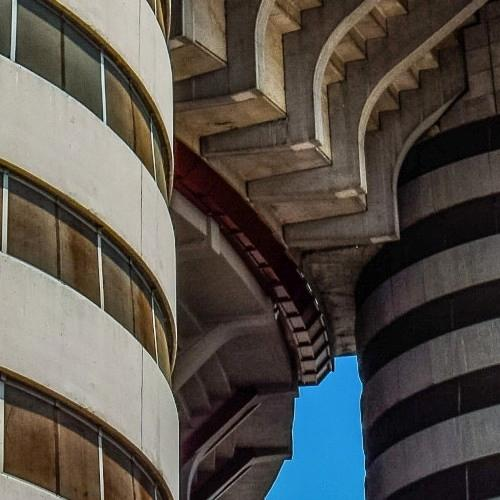
\includegraphics[width=\textwidth]{img/Original.jpg}
        \caption{Original}
    \end{subfigure}
    \hfill
    \begin{subfigure}[b]{0.24\textwidth}
        
\includegraphics[width=\textwidth]{img/Blur.jpg}
        \caption{Lighting}
        \label{fig:lighting}
    \end{subfigure}
    \hfill
    \begin{subfigure}[b]{0.24\textwidth}
        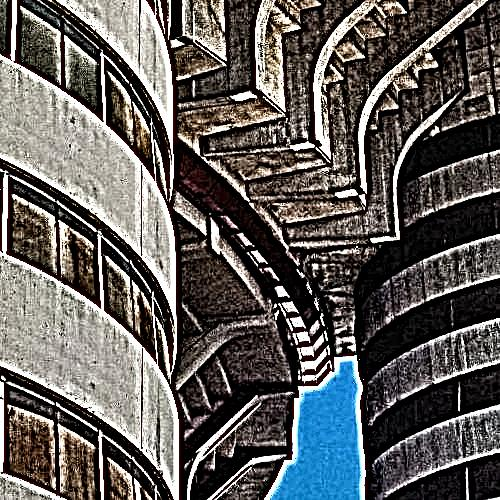
\includegraphics[width=\textwidth]{img/Sharpness.jpg}
        \caption{Background}
        \label{fig:background}
    \end{subfigure}
    \hfill
    \begin{subfigure}[b]{0.24\textwidth}
        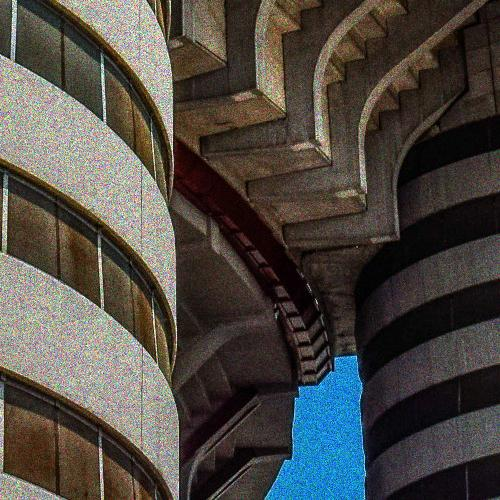
\includegraphics[width=\textwidth]{img/Noise.jpg}
        \caption{Field of View}
        \label{fig:FoV}
    \end{subfigure} 

    \begin{subfigure}[b]{0.24\textwidth}
        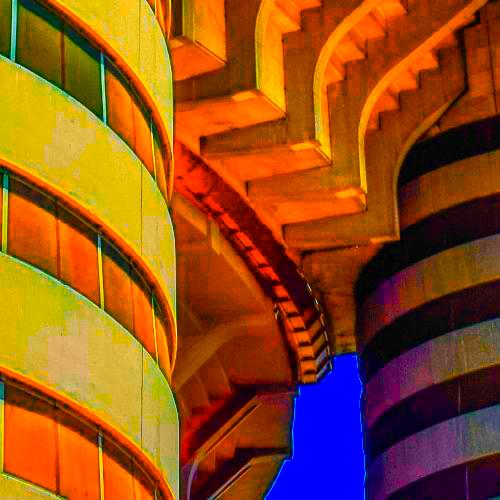
\includegraphics[width=\textwidth]{img/ColorAccuracy.jpg}
        \caption{Orientation}
        \label{fig:orientation}
    \end{subfigure}
    \hfill
    \begin{subfigure}[b]{0.24\textwidth}
        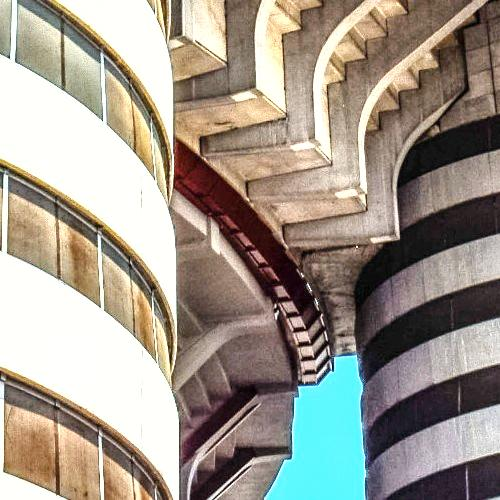
\includegraphics[width=\textwidth]{img/BrightnessContrast.jpg}
        \caption{Focus}
        \label{fig:focus}
    \end{subfigure}
    \hfill
    \begin{subfigure}[b]{0.24\textwidth}
        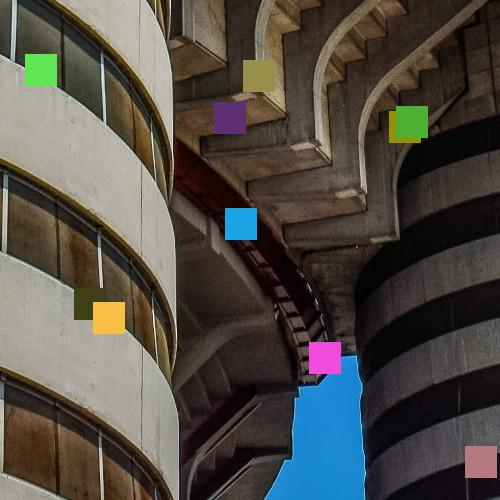
\includegraphics[width=\textwidth]{img/Artifacts.jpg}
        \caption{Resolution}
        \label{fig:resol}
    \end{subfigure}
    \hfill
    \begin{subfigure}[b]{0.24\textwidth}
        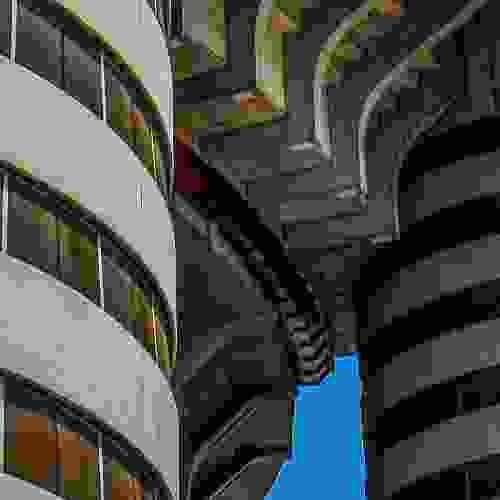
\includegraphics[width=\textwidth]{img/Compression.jpg}
        \caption{Color Calibration}
        \label{fig:cc}
    \end{subfigure}
    \caption{Example images illustrating common distortions used in Teledermatology Image Quality Assessment.}
    \label{fig:quality_criteria}
\end{figure}
\begin{enumerate}
    \item \textbf{Lighting}:  Adequate illumination is critical. It should be even and diffuse, avoiding harsh shadows or overexposure that could obscure skin lesions or lead to misinterpretation of the skin's condition. \textbf{Remark} Position the light source evenly to avoid shadows and overexposure. Natural light or diffused artificial light can help illuminate the skin lesion uniformly and reduce glare.
    \item \textbf{Background}: A neutral and uncluttered background helps to focus attention on the dermatological issue without distraction, ensuring that the skin lesion is the most prominent feature in the image. \textbf{Remark} Use a plain, non-reflective background to minimize distractions and ensure the focus remains on the skin lesion. A neutral-colored backdrop, such as white or gray, is ideal for providing contrast with the lesion.
    \item \textbf{Field of View}: The image should be framed to include a clear view of the lesion as well as sufficient surrounding area to provide context, which can be crucial for accurate diagnosis. \textbf{Remark} Center the skin lesion or area of interest within the frame to ensure complete coverage and avoid cutting off important details. Maintain a consistent distance between the camera and the skin to prevent distortion.
    \item \textbf{Orientation}: Proper orientation of the image is vital. It should align with standard anatomical positions, allowing the dermatologist to easily interpret the image in relation to the patient's body. \textbf{Remark} Orient the camera perpendicular to the skin surface to capture images in the correct orientation. Align the camera with the skin lesion to maintain consistency and facilitate accurate comparison between images.
    \item \textbf{Focus \& Depth of Field}: Sharp focus on the lesion is a necessity, with a depth of field that keeps the entire area of interest in clear detail, as blurring can mask important characteristics of skin conditions. \textbf{Remark} Ensure the camera is in focus and adjust the aperture to achieve sufficient depth of field. Focus on the skin lesion to capture sharp, detailed images without blurriness or loss of clarity.
    \item \textbf{Resolution}: The image must be high resolution to reveal fine details of the skin. A higher pixel count can facilitate a more thorough examination and better clinical decision-making. \textbf{Remark} Use a camera with high-resolution capabilities to capture fine details and nuances of the skin lesion. Adjust the camera settings to the highest resolution possible to ensure clarity and precision in the image.
    \item \textbf{Color Calibration}:  Accurate color reproduction is necessary for the assessment of skin lesions. Any color distortion can lead to misdiagnosis, especially in conditions where hue is a diagnostic clue. \textbf{Remark} Calibrate the camera settings to accurately reproduce colors and skin tones. Avoid harsh lighting or color casts that may distort the color representation of the skin lesion. Use a color reference chart or white balance settings to ensure color accuracy.
\end{enumerate}
Each of these quality criteria contributes to the diagnostic accuracy in teledermatology by ensuring that the images convey the true nature of the skin condition. Just as in traditional dermatology, where the dermatologist's visual assessment is a key diagnostic tool, in teledermatology, the image serves as the eyes of the dermatologist. Therefore, optimizing these criteria is crucial to the successful application of teledermatology services.


\subsection{Teledermatology Datasets}
\label{sub:DatasetsTD}
The following datasets are valuable resources for teledermatology research and applications, especially notable for their accessibility and diversity. These datasets are not strictly confined to clinical settings or dermoscopic images and include patient-taken images, making them highly relevant for practical teledermatology purposes where clinical settings may vary:
\begin{itemize}
    \item \textbf{ACNE04}: This dataset focuses on acne severity and lesion counting, containing 1,457 images with detailed annotations for training and testing purposes (\cite{ACNE04}).
    \item \textbf{DDI}: Provides 656 high-quality images curated by dermatologists for detailed skin tone evaluation and diagnostic accuracy (\cite{DDI}).
    \item \textbf{Derm7pt}: Utilizes 1,011 lesion cases to train a neural network for classifying skin lesions and melanoma using the 7-point checklist (\cite{Derm7pt}).
    \item \textbf{Fitzpatrick17k}: Includes 16,577 images annotated for Fitzpatrick skin type across 114 different skin conditions (\cite{F17K}).
    \item \textbf{Monkeypox Dataset 2022}: Contains approximately 1,905 images focused on monkeypox, useful for developing diagnostic tools (\cite{Monkeypox}).
    \item \textbf{PAD-UFES-20}: Comprises 2,298 clinical images from smartphones, enriched with clinical metadata for comprehensive research (\cite{PAD-UFES-20}).
    \item \textbf{SCIN}: Emerged from a crowdsourcing initiative, this dataset contains 10,408 images capturing a broad spectrum of dermatological conditions (\cite{SCIN}).
\end{itemize}
\vspace{\baselineskip}
\noindent
These datasets collectively contribute to the advancement of teledermatology by providing varied, real-world data crucial for developing effective diagnostic tools and algorithms. \par 

\subsection{Approaches to Image Quality Assessment in Teledermatology}
\label{sub:ApproachesIQAinTeledermatology}
To understand the various approaches to Image Quality Assessment (IQA) within teledermatology, it is instructive to review related works that have contributed to the field. These studies not only offer insights into the methodologies employed for assessing image quality but also highlight the specific image distortions that are often targeted. Furthermore, by examining the architectures of the algorithms and the criteria used to classify image quality, we can discern the strengths and weaknesses of each approach. \par

\subsubsection{TrueImage: A Machine Learning Algorithm to Improve the Quality of Telehealth Photos}
\label{subsub:TrueImage}
The TrueImage algorithm prioritizes real-time, interactive feedback for patients taking dermatological images via their smartphones. Its three-stage process includes semantic segmentation to identify skin regions, feature generation focusing on blur, lighting, and zoom, and logistic regression classifiers that predict image quality and specific reasons for poor quality (\cite{TrueImage}). \par
\vspace{\baselineskip}
\noindent
The prototype exhibits promise, demonstrating the capability to reject approximately half of sub-par quality images while retaining around 80\% of good quality images. This suggests its potential utility in a clinical setting, where it could save time for both clinicians and patients by pre-screening image quality and offering specific feedback to improve poor submissions (\cite{TrueImage}).
\par
\vspace{\baselineskip}
\noindent
Yet, TrueImage’s current limitation lies in its modest dataset and the training data's lack of diversity regarding skin types, which could lead to biased quality assessments. Furthermore, while the algorithm excels at detecting blurriness, it is less effective at assessing lighting conditions and zoom, which are critical factors in teledermatology (\cite{TrueImage}).\par

\subsubsection{ImageQX: Explainable Image Quality Assessments in Teledermatological Photography}
\label{subsub:ImageQX}
ImageQX offers an automated, deployable method for IQA in teledermatology, addressing common image distortions: such as poor framing, bad lighting, blur, low resolution, and distance issues. With an architecture that employs the EfficientNet-B0 as a lightweight feature extractor. The network then employs linear layers, batch normalization, and dropout layers to predict poor image quality reasons, integrating them to forecast overall image quality (\cite{ImageQX}).
\par
\vspace{\baselineskip}
\noindent
The approach is data-driven, validated on a substantial dataset annotated by dermatologists, which underscores its potential for real-world applicability. With a macro F1-score of 0.73 for image quality assessment, ImageQX demonstrates expertise comparable to dermatologists and a capability for explainability via attention maps that can guide patients to retake pictures more effectively (\cite{ImageQX}).
\par
\vspace{\baselineskip}
\noindent
However, while ImageQX achieves high specificity, suggesting minimal disruption to patient experience by incorrectly rejecting high-quality images, its predictive performance for certain poor quality explanations like 'bad framing' remains low, with an F1-score of 0.37 (\cite{ImageQX}). This indicates room for improvement in addressing certain types of distortions, though the network’s size (15MB) makes it an attractive option for mobile deployment.
\par
\vspace{\baselineskip}
\vspace{\baselineskip}
\noindent
ImageQX stands out with its deep learning approach that uses a convolutional neural network (CNN) trained on a dataset of images labeled for quality by board-certified dermatologists. The network architecture is based on the lightweight EfficientNet-B0, which facilitates deployment on mobile devices. This model's training utilized a large dataset of 36,509 images, where the photographs were annotated for common quality issues, such as framing, lighting, blur, resolution, and distance from the subject.
\par
\noindent
\vspace{\baselineskip}
The strength of ImageQX lies in its explainability and its ability to provide reasons for poor image quality, aligning closely with the common distortions identified by dermatologists. It achieves a high macro F1-score, suggesting that its performance in image quality assessment is on par with expert human raters. However, some limitations include the difficulty of explaining certain quality issues like 'blurry' images, which had lower inter-rater agreement scores. The model's reliance on dermatologist-annotated images also points to the importance of the quality and diversity of the training dataset for its generalizability and accuracy. \par
\noindent
\vspace{\baselineskip}
In conclusion, both ImageQX and TrueImage present pioneering steps towards automated IQA in teledermatology, each with strengths such as deployability and real-time feedback capabilities. Their current challenges include the need for more diverse training data, improved detection of certain distortions, and further validation in real-world settings. Addressing these challenges will be crucial for their successful integration into teledermatological practices, ultimately contributing to more efficient and effective remote dermatological care. \par

\subsection{Challenges and Opportunities in Teledermatology}
\label{sub:ChallengesOpportunitiesTeledermatology}
Teledermatology has fundamentally changed how dermatological care is accessed, particularly in remote or underserved areas. However, the field faces several challenges that intersect with the focus of this thesis on image quality assessment.\par
\noindent
\vspace{\baselineskip}
One major challenge is the variability in image quality, which stems from patients using a wide range of devices in uncontrolled environments to capture images. This variability can severely impact the consistency and reliability of diagnoses made remotely. Additionally, technological barriers such as disparities in access to high-quality digital devices and varying levels of digital literacy among patients can further affect the quality of submitted images. Moreover, ensuring the privacy and security of sensitive dermatological images transmitted over the internet remains a critical concern that needs continuous attention to safeguard patient data.\par
\noindent
\vspace{\baselineskip}
On the opportunity front, recent advancements in image processing and machine learning technologies present significant potential to automatically enhance image quality and correct common distortions. This can greatly aid in improving diagnostic accuracy and efficiency. There is also a considerable opportunity to develop and implement standardized guidelines for image capture in teledermatology. Such standardization can help minimize quality variability and streamline the diagnostic process. Furthermore, the integration of artificial intelligence to provide real-time feedback to patients on improving image quality can enhance the effectiveness of teledermatology services by ensuring that only high-quality images are evaluated by dermatologists.\par
\noindent
\vspace{\baselineskip}
By tackling these challenges and leveraging the emerging opportunities, teledermatology can continue to evolve and play a crucial role in modern healthcare, enhancing access and efficiency in dermatological care across diverse populations.\par